\label{sec:evaluation}

We use a subset of the Duets benchmarks~\cite{durieux21} comprising 
10 libraries and their clients, totalling to 85 software projects. We have 
collected both static and dynamic data for these projects.

\begin{figure*}[h]
\begin{center}
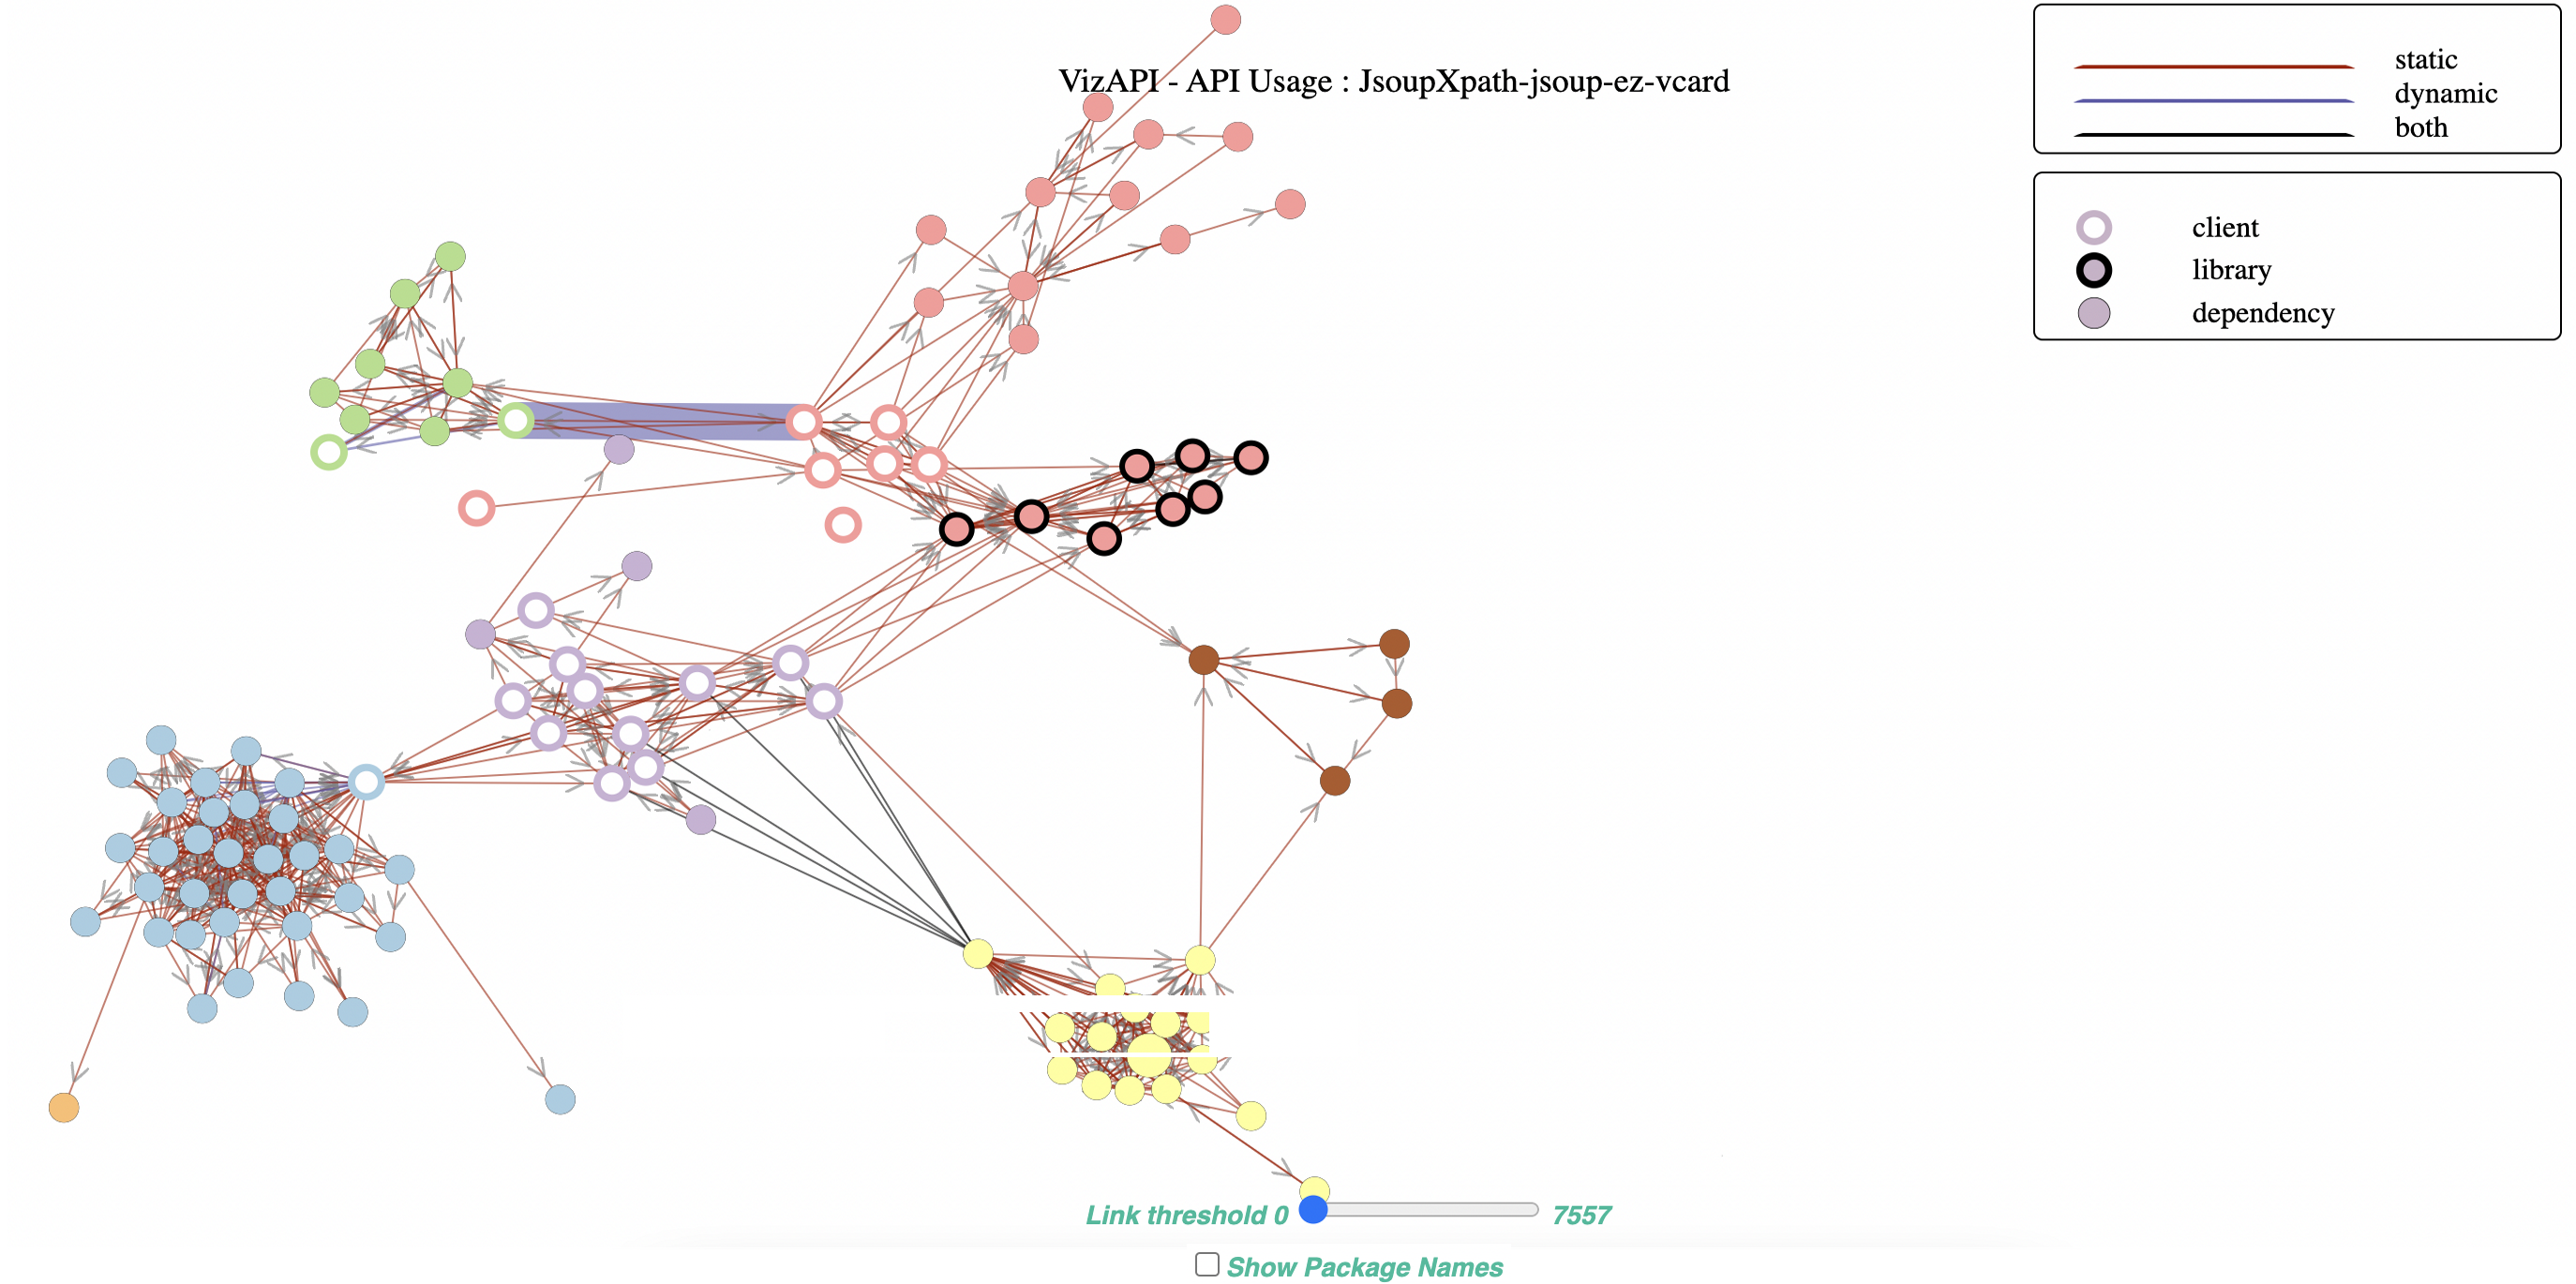
\includegraphics[scale=1,width=18cm,height=8cm]{images/usage-scenario1.png}
\caption{Usage Scenario 1 : jsoup(library), JsoupXpath(client), ez-vcard(client)}
\label{fig:usagescenario1}
\end{center}
\end{figure*}

Now, we walk through an example usage scenario of VizAPI.
The graph in Figure~\ref{fig:usagescenario1} represents the static and dynamic interactions of JsoupXpath\footnote{\url{https://github.com/zhegexiaohuozi/JsoupXpath}\label{jsoupxpath}} and ez-vcard\footnote{\url{https://github.com/mangstadt/ez-vcard}\label{ez-vcard}}, which we are visualizing as clients. These clients call into jsoup\footnote{\url{https://github.com/jhy/jsoup}\label{jsoup}}, which is the library we look at.

We can start our exploration with the cluster of pink nodes. Many of these nodes belong to JsoupXpath\textsuperscript{\ref{jsoupxpath}} and jsoup\textsuperscript{\ref{jsoup}}. When we hover over them, the hover hints tell us that the client JsoupXpath\textsuperscript{\ref{jsoupxpath}} calls directly into \texttt{org.jsoup.nodes} and \texttt{org.jsoup.select}, but as we might expect, we see that \texttt{org.jsoup.helper} and \texttt{org.jsoup.internal} aren’t called directly by JsoupXpath\textsuperscript{\ref{jsoupxpath}}, as we might expect. This would mean that breaking changes in \texttt{org.jsoup.helper} or \texttt{org.jsoup.internal} wouldn’t directly affect JsoupXpath\textsuperscript{\ref{jsoupxpath}}. Similarly, ez-vcard\textsuperscript{\ref{ez-vcard}} directly calls into \texttt{org.jsoup}.

ez-vcard\textsuperscript{\ref{ez-vcard}} also calls into jackson-core\footnote{\url{https://github.com/FasterXML/jackson-core}\label{jackson-core}} and jackson-databind\footnote{\url{https://github.com/FasterXML/jackson-databind}\label{jackson-databind}}, which are very tightly coupled amongst their own packages and with each other. This could mean that breaking changes in these libraries can propagate to many of their own packages.
.

